\documentclass{beamer}

% xcolor and define colors -------------------------
\usepackage{xcolor}

% https://www.viget.com/articles/color-contrast/
\definecolor{purple}{HTML}{5601A4}
\definecolor{navy}{HTML}{0D3D56}
\definecolor{ruby}{HTML}{9a2515}
\definecolor{alice}{HTML}{107895}
\definecolor{daisy}{HTML}{EBC944}
\definecolor{coral}{HTML}{F26D21}
\definecolor{kelly}{HTML}{829356}
\definecolor{cranberry}{HTML}{E64173}
\definecolor{jet}{HTML}{131516}
\definecolor{asher}{HTML}{555F61}
\definecolor{slate}{HTML}{314F4F}

% Mixtape Sessions
\definecolor{picton-blue}{HTML}{00b7ff}
\definecolor{violet-red}{HTML}{ff3881}
\definecolor{sun}{HTML}{ffaf18}
\definecolor{electric-violet}{HTML}{871EFF}

\newcommand\pictonBlue[1]{{\color{picton-blue}#1}}
\newcommand\sun[1]{{\color{sun}#1}}
\newcommand\electricViolet[1]{{\color{electric-violet}#1}}
\newcommand\violetRed[1]{{\color{violet-red}#1}}

\newcommand\bgPictonBlue[1]{{\colorbox{picton-blue!20!white}{#1}}}
\newcommand\bgSun[1]{{\colorbox{sun!20!white}{#1}}}
\newcommand\bgElectricViolet[1]{{\colorbox{electric-violet!20!white}{#1}}}
\newcommand\bgVioletRed[1]{{\colorbox{violet-red!20!white}{#1}}}

\def\code#1{\texttt{#1}}

% Main theme colors
\definecolor{accent}{HTML}{00b7ff}
\definecolor{accent2}{HTML}{871EFF}
\definecolor{gray100}{HTML}{f3f4f6}
\definecolor{gray800}{HTML}{1F292D}


% Beamer Options -------------------------------------

% Background
\setbeamercolor{background canvas}{bg = white}

% Change text margins
\setbeamersize{text margin left = 15pt, text margin right = 15pt} 

% \alert
\setbeamercolor{alerted text}{fg = accent2}

% Frame title
\setbeamercolor{frametitle}{bg = white, fg = jet}
\setbeamercolor{framesubtitle}{bg = white, fg = accent}
\setbeamerfont{framesubtitle}{size = \small, shape = \itshape}

% Block
\setbeamercolor{block title}{fg = white, bg = accent2}
\setbeamercolor{block body}{fg = gray800, bg = gray100}

% Title page
\setbeamercolor{title}{fg = gray800}
\setbeamercolor{subtitle}{fg = accent}

%% Custom \maketitle and \titlepage
\setbeamertemplate{title page}
{
    %\begin{centering}
        \vspace{20mm}
        {\Large \usebeamerfont{title}\usebeamercolor[fg]{title}\inserttitle}\\
        {\large \itshape \usebeamerfont{subtitle}\usebeamercolor[fg]{subtitle}\insertsubtitle}\\ \vspace{10mm}
        {\insertauthor}\\
        {\color{asher}\small{\insertdate}}\\
    %\end{centering}
}

% Table of Contents
\setbeamercolor{section in toc}{fg = accent!70!jet}
\setbeamercolor{subsection in toc}{fg = jet}

% Button 
\setbeamercolor{button}{bg = accent}

% Remove navigation symbols
\setbeamertemplate{navigation symbols}{}

% Table and Figure captions
\setbeamercolor{caption}{fg=jet!70!white}
\setbeamercolor{caption name}{fg=jet}
\setbeamerfont{caption name}{shape = \itshape}

% Bullet points

%% Fix spacing between items
\let\olditemize=\itemize 
\let\endolditemize=\enditemize 
\renewenvironment{itemize}{\vspace{0.25em}\olditemize \itemsep0.25em}{\endolditemize}

%% Fix left-margins
\settowidth{\leftmargini}{\usebeamertemplate{itemize item}}
\addtolength{\leftmargini}{\labelsep}

%% enumerate item color
\setbeamercolor{enumerate item}{fg = accent}
\setbeamerfont{enumerate item}{size = \small}
\setbeamertemplate{enumerate item}{\insertenumlabel.}

%% itemize
\setbeamercolor{itemize item}{fg = accent!70!white}
\setbeamerfont{itemize item}{size = \small}
\setbeamertemplate{itemize item}[circle]

%% right arrow for subitems
\setbeamercolor{itemize subitem}{fg = accent!60!white}
\setbeamerfont{itemize subitem}{size = \small}
\setbeamertemplate{itemize subitem}{$\rightarrow$}

\setbeamertemplate{itemize subsubitem}[square]
\setbeamercolor{itemize subsubitem}{fg = jet}
\setbeamerfont{itemize subsubitem}{size = \small}








% Links ----------------------------------------------

\usepackage{hyperref}
\hypersetup{
  colorlinks = true,
  linkcolor = accent2,
  filecolor = accent2,
  urlcolor = accent2,
  citecolor = accent2,
}


% Line spacing --------------------------------------
\usepackage{setspace}
\setstretch{1.35}


% \begin{columns} -----------------------------------
\usepackage{multicol}


% Fonts ---------------------------------------------
% Beamer Option to use custom fonts
\usefonttheme{professionalfonts}

% \usepackage[utopia, smallerops, varg]{newtxmath}
% \usepackage{utopia}
\usepackage[sfdefault,light]{roboto}

% Small adjustments to text kerning
\usepackage{microtype}



% Remove annoying over-full box warnings -----------
\vfuzz2pt 
\hfuzz2pt


% Table of Contents with Sections
\setbeamerfont{myTOC}{series=\bfseries, size=\Large}
\AtBeginSection[]{
        \frame{
            \frametitle{Roadmap}
            \tableofcontents[current]   
        }
    }


% Tables -------------------------------------------
% Tables too big
% \begin{adjustbox}{width = 1.2\textwidth, center}
\usepackage{adjustbox}
\usepackage{array}
\usepackage{threeparttable, booktabs, adjustbox}
    
% Fix \input with tables
% \input fails when \\ is at end of external .tex file
\makeatletter
\let\input\@@input
\makeatother

% Tables too narrow
% \begin{tabularx}{\linewidth}{cols}
% col-types: X - center, L - left, R -right
% Relative scale: >{\hsize=.8\hsize}X/L/R
\usepackage{tabularx}
\newcolumntype{L}{>{\raggedright\arraybackslash}X}
\newcolumntype{R}{>{\raggedleft\arraybackslash}X}
\newcolumntype{C}{>{\centering\arraybackslash}X}

% Figures

% \imageframe{img_name} -----------------------------
% from https://github.com/mattjetwell/cousteau
\newcommand{\imageframe}[1]{%
    \begin{frame}[plain]
        \begin{tikzpicture}[remember picture, overlay]
            \node[at = (current page.center), xshift = 0cm] (cover) {%
                \includegraphics[keepaspectratio, width=\paperwidth, height=\paperheight]{#1}
            };
        \end{tikzpicture}
    \end{frame}%
}

% subfigures
\usepackage{subfigure}


% Highlight slide -----------------------------------
% \begin{transitionframe} Text \end{transitionframe}
% from paulgp's beamer tips
\newenvironment{transitionframe}{
    \setbeamercolor{background canvas}{bg=accent!40!black}
    \begin{frame}\color{accent!10!white}\LARGE\centering
}{
    \end{frame}
}


% Table Highlighting --------------------------------
% Create top-left and bottom-right markets in tabular cells with a unique matching id and these commands will outline those cells
\usepackage[beamer,customcolors]{hf-tikz}
\usetikzlibrary{calc}
\usetikzlibrary{fit,shapes.misc}

% To set the hypothesis highlighting boxes red.
\newcommand\marktopleft[1]{%
    \tikz[overlay,remember picture] 
        \node (marker-#1-a) at (0,1.5ex) {};%
}
\newcommand\markbottomright[1]{%
    \tikz[overlay,remember picture] 
        \node (marker-#1-b) at (0,0) {};%
    \tikz[accent!80!jet, ultra thick, overlay, remember picture, inner sep=4pt]
        \node[draw, rectangle, fit=(marker-#1-a.center) (marker-#1-b.center)] {};%
}


% DAGS ----------------------------------------------
\usepackage{tikz}
\usetikzlibrary{shapes,decorations,arrows,calc,arrows.meta,fit,positioning}
% Tikz settings optimized for causal graphs.
\tikzset{
    -Latex,auto,node distance =1 cm and 1 cm,semithick,
    state/.style ={ellipse, draw, minimum width = 0.7 cm},
    point/.style = {circle, draw, inner sep=0.04cm,fill,node contents={}},
    bidirected/.style={Latex-Latex,dashed},
    el/.style = {inner sep=2pt, align=left, sloped}
}


% Beamer tricks -------------------------------------
% Make \pause work in align environments
\makeatletter
\renewrobustcmd{\beamer@@pause}[1][]{%
  \unless\ifmeasuring@%
  \ifblank{#1}%
    {\stepcounter{beamerpauses}}%
    {\setcounter{beamerpauses}{#1}}%
  \onslide<\value{beamerpauses}->\relax%
  \fi%
}
\makeatother




\begin{document}

\imageframe{./lecture_includes/cover_frontiers.png}

\section{Judge/Examiner IV}

\subsection{Approach}
\begin{frame}{Approach}
\vspace{-0.2cm}
A judge (or examiner) IV design leverages the idiosyncratic assignment of individuals to a set of decision-makers\smallskip
\begin{itemize}
\item Kling (2006): sentencing judges\smallskip
\item Doyle (2007): foster care investigators\smallskip
\item Maestas et al. (2013): SSDI benefit examiners\smallskip
\item Doyle et al. (2015): ambulance companies
\end{itemize}\bigskip\pause{}
The typical approach is to IV a treatment $D_i$ with a measure of the ``leniency'' $E[D_i\mid Z_{i}]$ of one's assigned judge $Z_i\in\{1,\dots,J\}$\smallskip
\begin{itemize}
\item E.g. a leave-one-out average, $\hat{L}_i=\frac{1}{|i^\prime\neq i,Z_{i^\prime}=Z_i|}\sum_{i^\prime \neq i,Z_{i^\prime}=Z_i}D_i$
\end{itemize}
\end{frame}

\begin{frame}{Agan et al. (2021) ``Misdemeanor Prosecution''}
\begin{center}
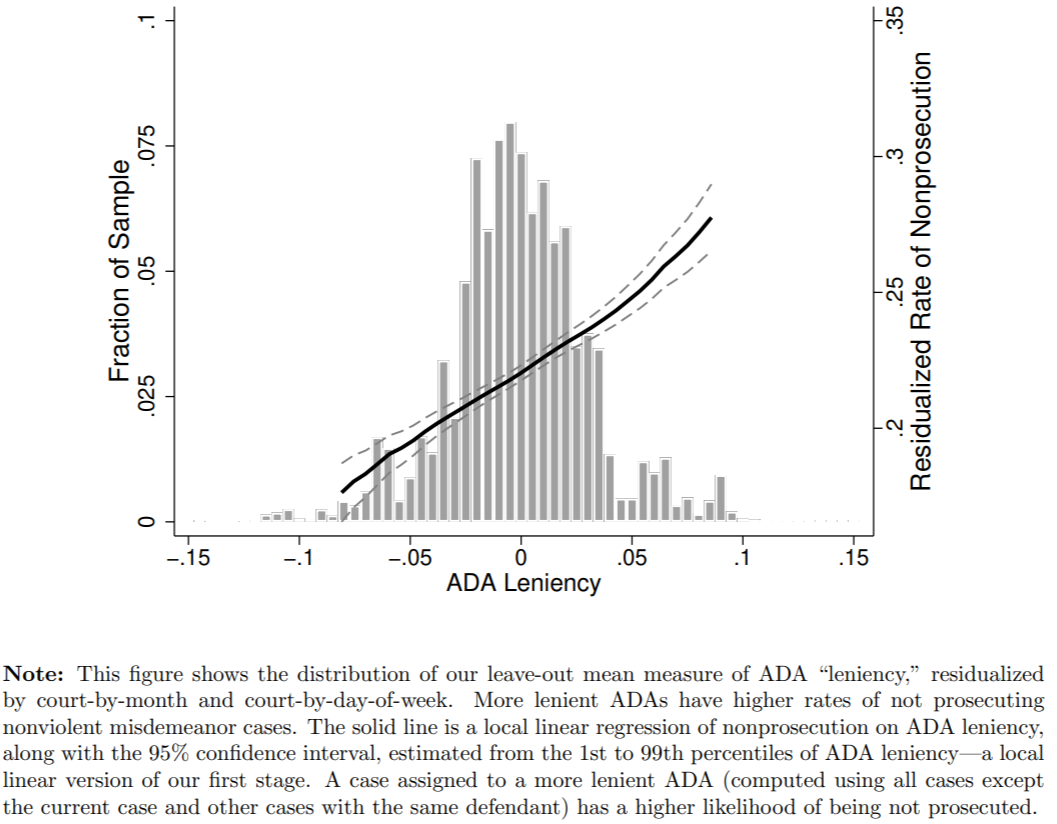
\includegraphics[scale=0.55]{./lecture_includes/agan_FS.png}
\end{center}
\end{frame}

\begin{frame}{Agan et al. (2021) ``Misdemeanor Prosecution''}
\vspace{-0.3cm}
\begin{center}
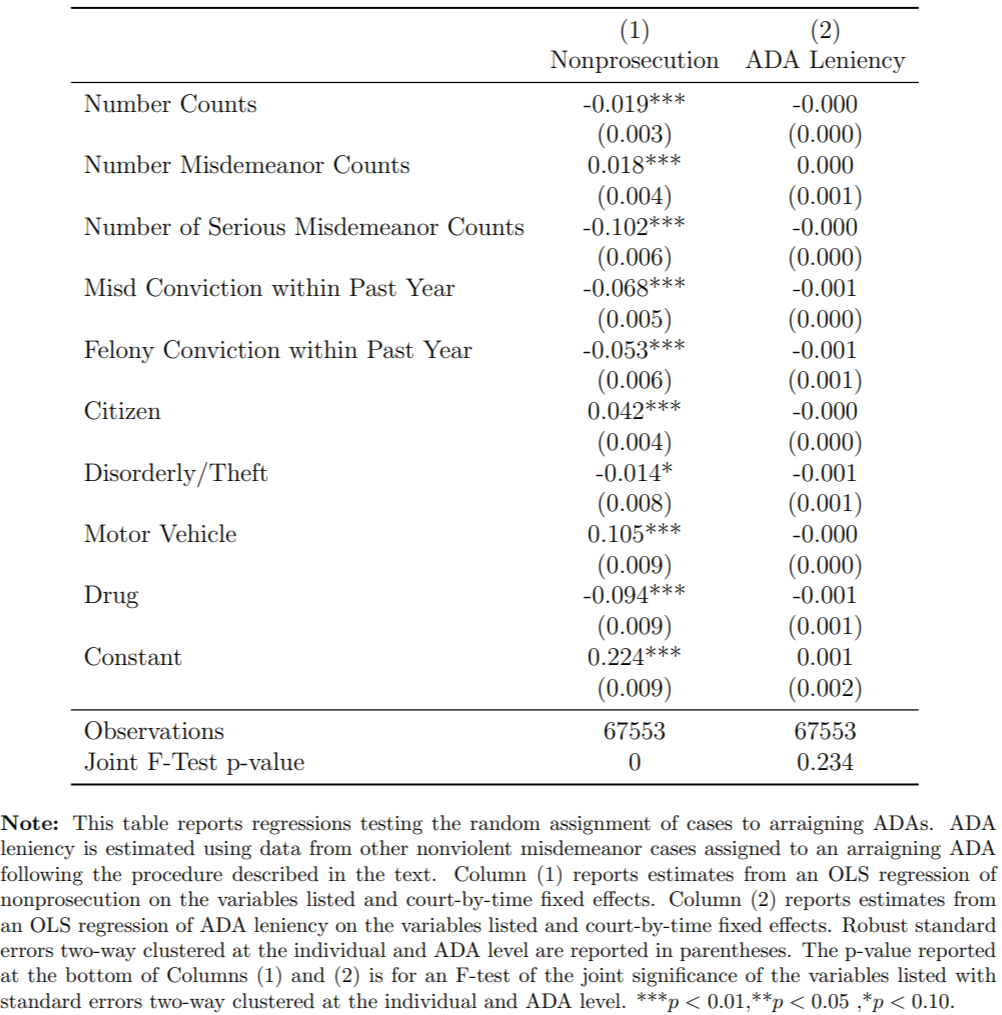
\includegraphics[scale=0.45]{./lecture_includes/agan_balance.png}
\end{center}
\end{frame}

\begin{frame}{Agan et al. (2021) ``Misdemeanor Prosecution''}
\vspace{-0.3cm}
\begin{center}
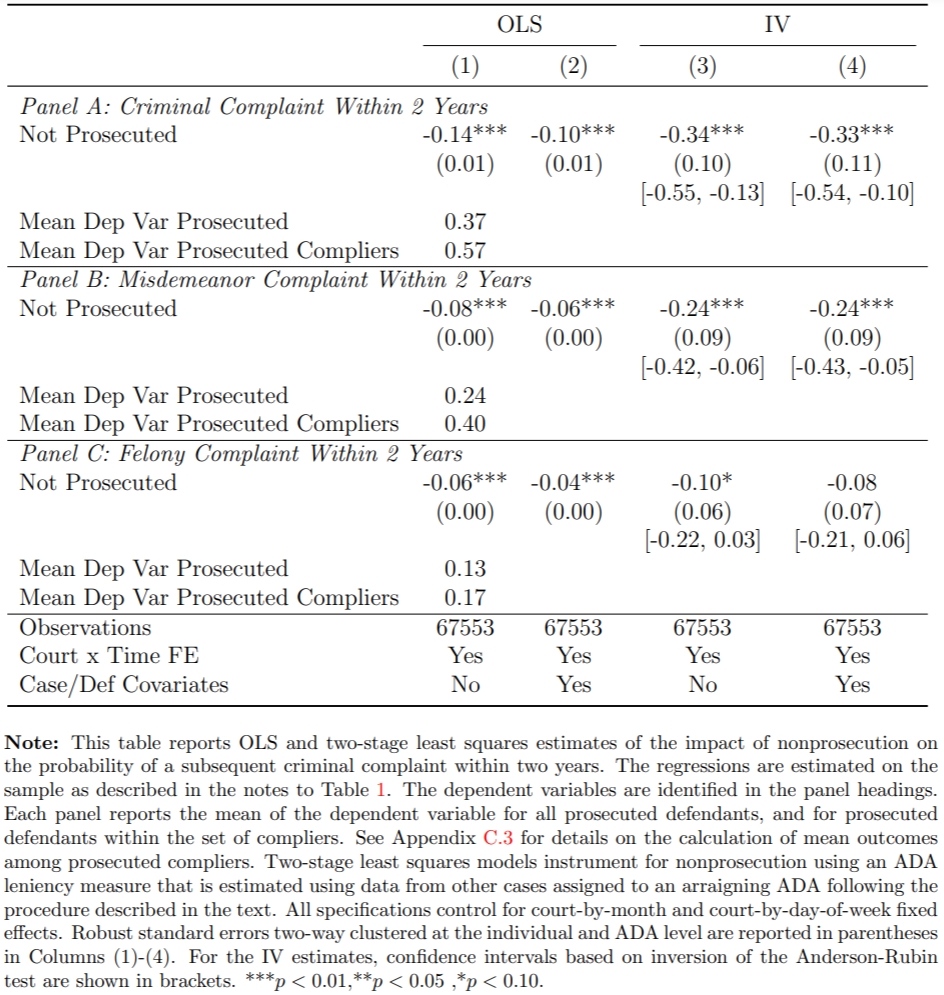
\includegraphics[scale=0.45]{./lecture_includes/agan_SS.png}
\end{center}
\end{frame}

\subsection{Cautions}
\begin{frame}{Caution 1: Monotonicity}
``Strict'' first-stage monotonicity requires judges to have a common ordering of individuals for treatment\smallskip
\begin{itemize}
\item E.g. no differences in ``skill'' at identifying appropriate cases
\end{itemize}\medskip\pause{}
Imbens and Angrist (\& Ridder) saw this coming in 1994! 
\begin{center}
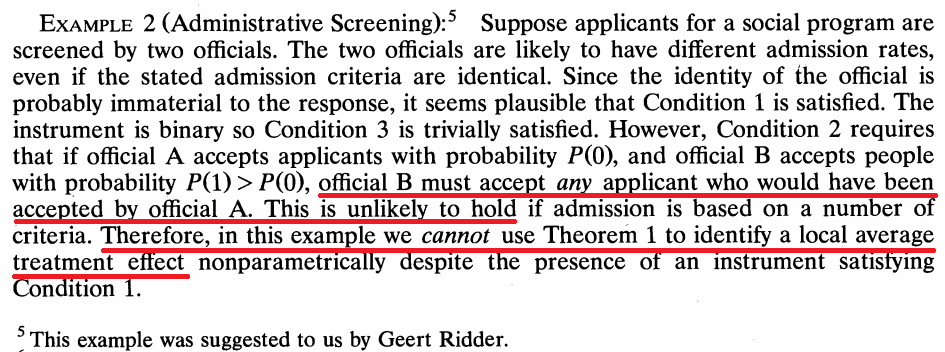
\includegraphics[scale=0.85]{./lecture_includes/imbens_angrist_judges.png}
\end{center}
\end{frame}

\begin{frame}{Monotonicity Solutions}
Frandsen et al. (2019) formalize a weaker ``average monotonicity'' condition: intuitively, that skill differences are uncorrelated with TEs\smallskip
\begin{itemize}
\item Similar to de Chaisemartin (2017) ``tolerating defiance''\smallskip
\item Also propose non-parametric tests of monotonicity + exclusion (similar to Kitagawa (2015), but with multiple IVs + controls)
\end{itemize}\medskip\pause{}

Other tests include checking whether leniency has the same first stage in different subgroups (Norris, 2021)\smallskip
\begin{itemize}
\item Another solution is to parameterize variation in judge skill and estimate it jointly with TEs (Chan et al. 2021; Arnold et al. 2021)
\end{itemize}

\end{frame}

\begin{frame}{Caution 2: Exclusion}
``Strict'' exclusion requires judges to only affect the outcome through one treatment channel\smallskip
\begin{itemize}
\item E.g. a judge more likely to sentence a defendant to jail does not differentially change sentence conditions
\end{itemize}\medskip\pause{}
Like monotonicity, this can be weakened to an ``on average'' condition\medskip
\begin{itemize}
\item Koles\'{a}r et al. (2015): exclusion restriction violations are uncorrelated with leniency variation (see also Angrist et al. 2021)\smallskip
\item Need many judges for a ``judge-level law of large numbers'' to kick in
\end{itemize}
\end{frame}

\begin{frame}{Adding Treatment Channels}
Of course if multiple potential treatment channels are observed they can be included + instrumented by judges\smallskip
\begin{itemize}
\item See Autor/Maestas/Mullen/Strand (2017), which adds a decision-time treatment to Maestas et al. (2013)\smallskip
\item Two instruments: examiner leniency and (leave-out) average examiner decision time
\end{itemize}\medskip\pause{}
Careful though: IV with multiple treatments can be difficult to interpret in a LATE framework (maybe OK as a robustness check)\smallskip
\begin{itemize}
\item See e.g. Kirkeboen et al. (2016) and Kline and Walters (2016)
\end{itemize}

\end{frame}

\begin{frame}{Caution 3: Leniency Estimation}
One concern that doesn't get enough attention (IMO) is the fact that judge leniency is estimated: after all, we don't know $E[D_i\mid Z_i]$!\smallskip\pause{}
\begin{itemize}
\item Estimating leniency as (non-leave-out) sample averages == using 2SLS with judge dummies (recall the ``2S'' in ``2SLS'!')\smallskip\pause{}
\item For leave-out averages, the equivalent regression uses Jacknife Instrumental Variables Estimation (JIVE; Angrist et al. 1999)
\end{itemize}\medskip\pause{}
JIVE may be better with many judge instruments (as it can avoid 2SLS many-weak bias), but it is not bulletproof\smallskip
\begin{itemize}
\item Koles\'{a}r (2013) shows many-weak bias can creep back in with many covariates (e.g. court-by-time FE, needed to make judges random)
\end{itemize}
\end{frame}

\begin{frame}{State-of-the-Art: UJIVE}
 Koles\'{a}r (2013) also derives a solution to many-IV/many-control bias \smallskip
\begin{itemize}
\item ``Unbiased'' Jackknife Instrumental Variables Estimation (UJIVE) adjusts the leave-out means for controls by (basically) leave-out-Frisch-Waugh-Lovell residualization
\end{itemize}\bigskip\pause{}
Michal Koles\'{a}r, Paul Goldsmith-Pinkham, and I are currently working on a Stata package to implement UJIVE  \smallskip
\begin{itemize}
\item We hope to publish it and an accompanying R package soon! In the meantime you'll be one of the first to beta-test our current code...
\end{itemize}
\end{frame}

\begin{frame}{UJIVE Repo (In Progress)}
\begin{center}
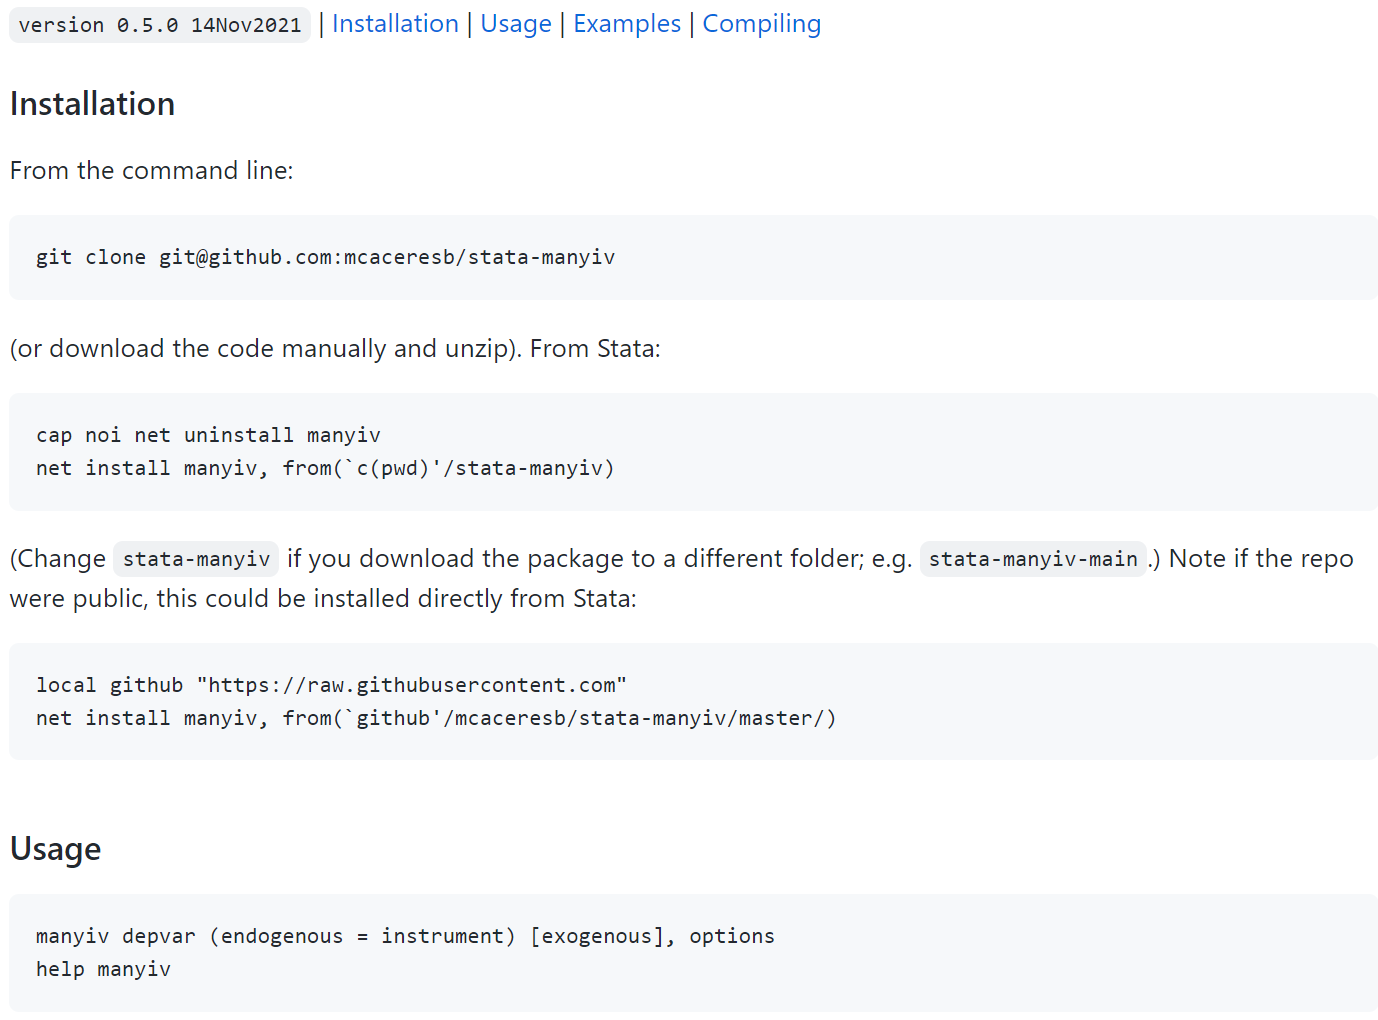
\includegraphics[scale=0.45]{./lecture_includes/manyiv.png}
\end{center}
\end{frame}



\section{Shift-Share IV}

\subsection{Approach}
\begin{frame}{Approach}
A shift-share instrument takes the form $Z_i=\sum_n \electricViolet{s_{in}} \sun{g_n}$ for a set of \bgSun{shocks} $\sun{g_n}$ and a set of \bgElectricViolet{exposure shares} $\electricViolet{s_{in}}\ge 0$ (for each $i$)\smallskip\pause{}
\begin{itemize}
  \item Bartik (1991): \sun{national industry employment growth} $\sun{g_n}$, \electricViolet{local industry employment shares} $\electricViolet{s_{in}}$ for regions $i$\smallskip
  \item Autor et al. (2013): \sun{increase in (non-U.S.) Chinese import growth across manufacturing industries} $\sun{g_n}$, \electricViolet{local employment shares} $\electricViolet{s_{in}}$\smallskip
  \item Card (2009): \sun{growth of immigrant inflows across origin countries} $\sun{g_n}$, \electricViolet{local immigrant shares} $\electricViolet{s_{in}}$
\end{itemize}\medskip\pause{}
The literature has taken two econometric approaches to such $Z_i$...
\end{frame}

\begin{frame}{Exogenous Shares}
Goldsmith-Pinkham et al. (2020) consider the shocks $\sun{g_n}$ as fixed numbers and consider the ``exogeneity'' of the shares: $E[\electricViolet{s_{in}}\varepsilon_i]=0$\smallskip
\begin{itemize}
  \item Often regressions are run in first-differences, so this is like DD-IV\smallskip
  \item The twist here is we have many instruments: In Autor et al. (2013) there are $398$ industries $n$ (and $1,444$ regional observations!)
\end{itemize}\bigskip\pause{}

They propose tools to measure the ``importance'' of different share IVs (``Rotemberg weights'') and discuss other subtlties in estimation\smallskip
\begin{itemize}
  \item Kind of like judge IV, except with known ``leniency'' $\sun{g_n}$\smallskip
  \item Can check (many) overidentifying restrictions, pre-trends, etc
\end{itemize}

\end{frame}

%\begin{frame}{Rotemberg Weights for Card (2009) Exposure Shares}
%\begin{center}
%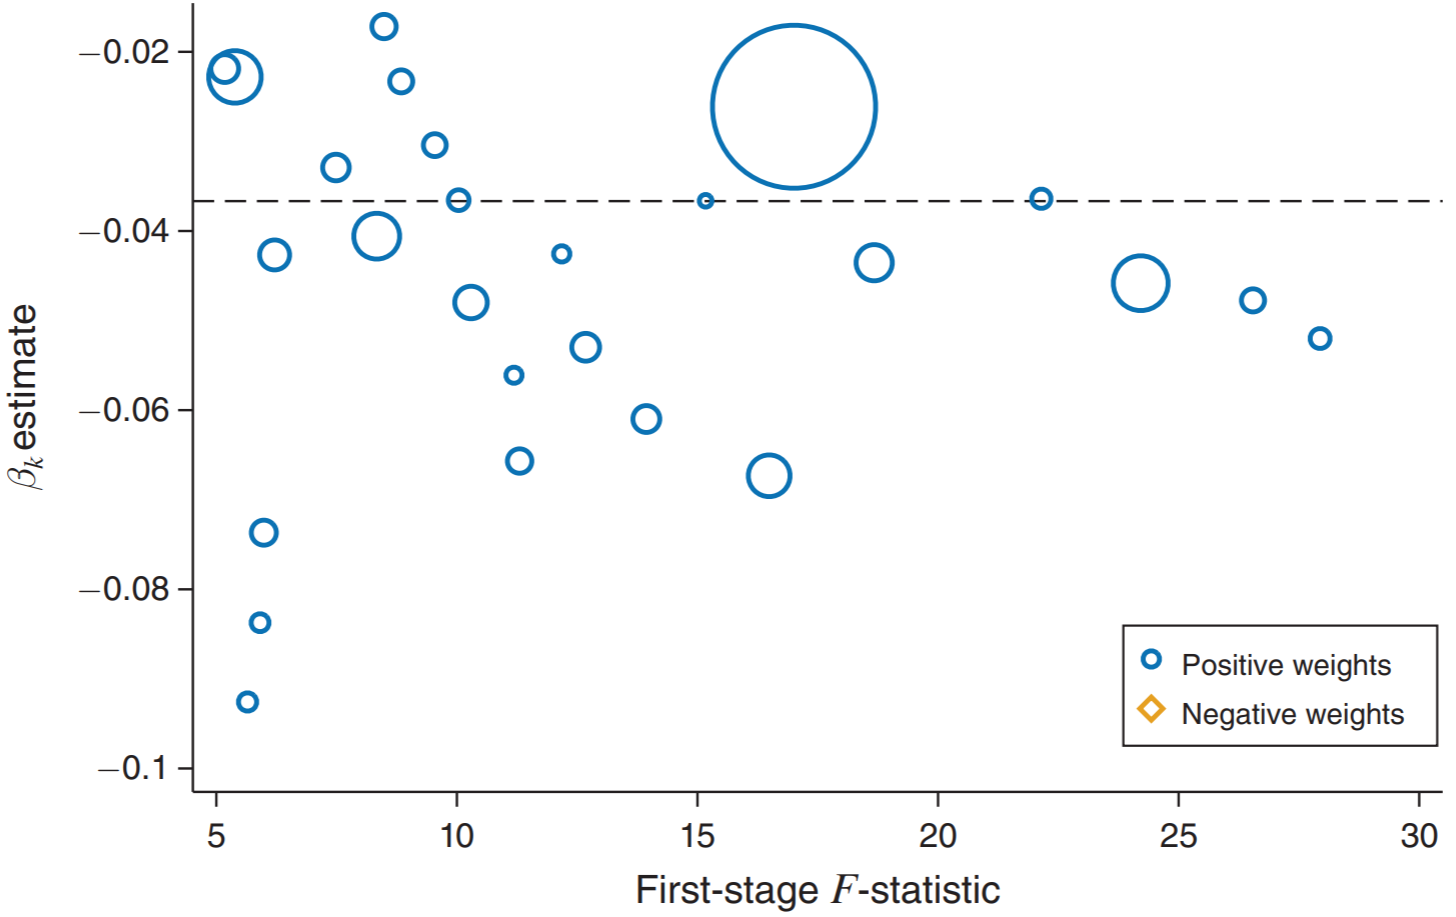
\includegraphics[scale=0.28]{./lecture_includes/card_weights.png}
%\end{center}
%\vspace{-0.3cm}
%Source: Goldsmith-Pinkham et al. (2020)
%\end{frame}

\begin{frame}{Exogenous Shocks}
Borusyak et al. (2022) consider the shocks $\sun{g_n}$ as exogenous,  (quasi-randomly assigned + excludable), conditional on the shares\smallskip
\begin{itemize}
  \item E.g. different industries saw higher/lower import growth from China for reasons unrelated to local U.S. employment trends\smallskip
  \item Need a ``shock-level law of large numbers'' (i.e. many shocks)
\end{itemize}\bigskip\pause{}

They propose tools to test for shock exogeneity (e.g. balance/ pre-trend checks) and quantify the extent of identifying variation \smallskip
\begin{itemize}
  \item No overidentifying restrictions: a single instrument $\sun{g_n}$, as if we were running an ``industry-level'' IV regression \smallskip
  \item Also show how to relax exogeneity to hold conditional on some observed shock-level confounders
\end{itemize}

\end{frame}


%\subsection{Cautions}
%\begin{frame}{Caution 1: Incomplete Shares}
%In some shift-share applications exposure weight sum $S_i=\sum_n \electricViolet{s_{in}}$ varies across observations $i$\smallskip
%\begin{itemize}
%\item E.g. in Autor et al. (2013), the total manufacturing share $S_i$ varies
%\end{itemize}\medskip\pause{}
%Borusyak et al. (2022) show this can be a problem if you only want to leverage variation in the shocks and not also in $S_i$ \smallskip
%\begin{itemize}
%\item Intuitively, if $E[\sun{g_n}|s]=\mu$ then $E[Z_i|s]=E\left[\sum_n \electricViolet{s_{in}}\sun{g_n}|s\right]=\mu S_i$, so the ``expected instrument'' varies non-randomly across observations\smallskip
%\item If $S_i$ is correlated with $\varepsilon_i$, this non-random variation can create bias
%\end{itemize}
%\end{frame}

%\begin{frame}{Addressing Incomplete Shares}
%An easy fix to incomplete shares is to control for $S_i=\sum_n \electricViolet{s_{in}}$\smallskip
%\begin{itemize}
%\item Alternatively, construct shares such that $S_i=1$ for everyone\smallskip
%\item The former may be more powerful if $X_i=\sum_n \electricViolet{s_{in}} \tilde{g}_{in}$ for $S_i\neq 1$
%\end{itemize}\medskip\pause{}
%If other controls are needed to make the shocks as-good-as- random (e.g. time dummies, to isolate within-period variation) then $S_i$ needs to be added as an \emph{interaction} with them\smallskip
%\begin{itemize}
%\item In Autor et al. (2013), this means interacting the manufacturing sum-of-shares with period FE...
%\end{itemize}
%\end{frame}

%\begin{frame}{Sum-of-Share Controls in Autor et al. (2013)}
%\vspace{-0.3cm}
%\begin{center}
%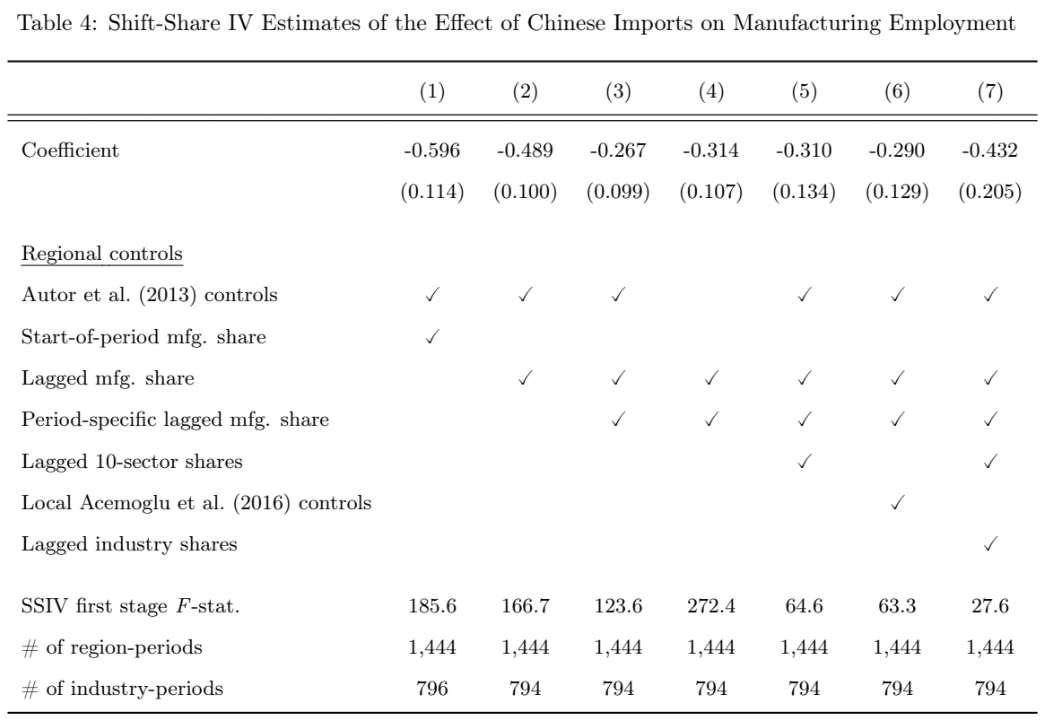
\includegraphics[scale=0.4]{./lecture_includes/adh_bhj.png}
%\end{center}
%\vspace{-0.3cm}
%Source: Borusyak et al. (2022)
%\end{frame}

%\begin{frame}{Caution 2: Exposure Clustering}
%Ad\'{a}o et al. (2019) show another problem with exogenous shocks: conventional robust/clustered SEs may be wrong \smallskip
%\begin{itemize}
%\item Intuitively, the structure of $Z_{i}=\sum_n \electricViolet{s_{in}}\sun{g_n}$ may make observations with similar $\electricViolet{s_{i1} \dots s_{in}}$ correlated, even when otherwise ``far apart''\smallskip
%\item They derive non-standard central limit theorems to account for such ``exposure clustering'' (with R/Stata code)
%\end{itemize}\medskip\pause{}
%Borusyak et al. (2022) build on this theory to propose an alternative approach: estimate the IV at the level of identifying variation (shocks)\smallskip
%\begin{itemize}
%\item Derive an equivalent regression where the $\sun{g_n}$ are used directly as the instrument for shock-level outcomes and treatments\smallskip
%\item Standard robust SEs address the exposure clustering problem
%\end{itemize}

%\end{frame}

\begin{frame}{Estimating Exogenous-Shock SSIV Regressions in Stata}
\vspace{-0.3cm}
\begin{center}
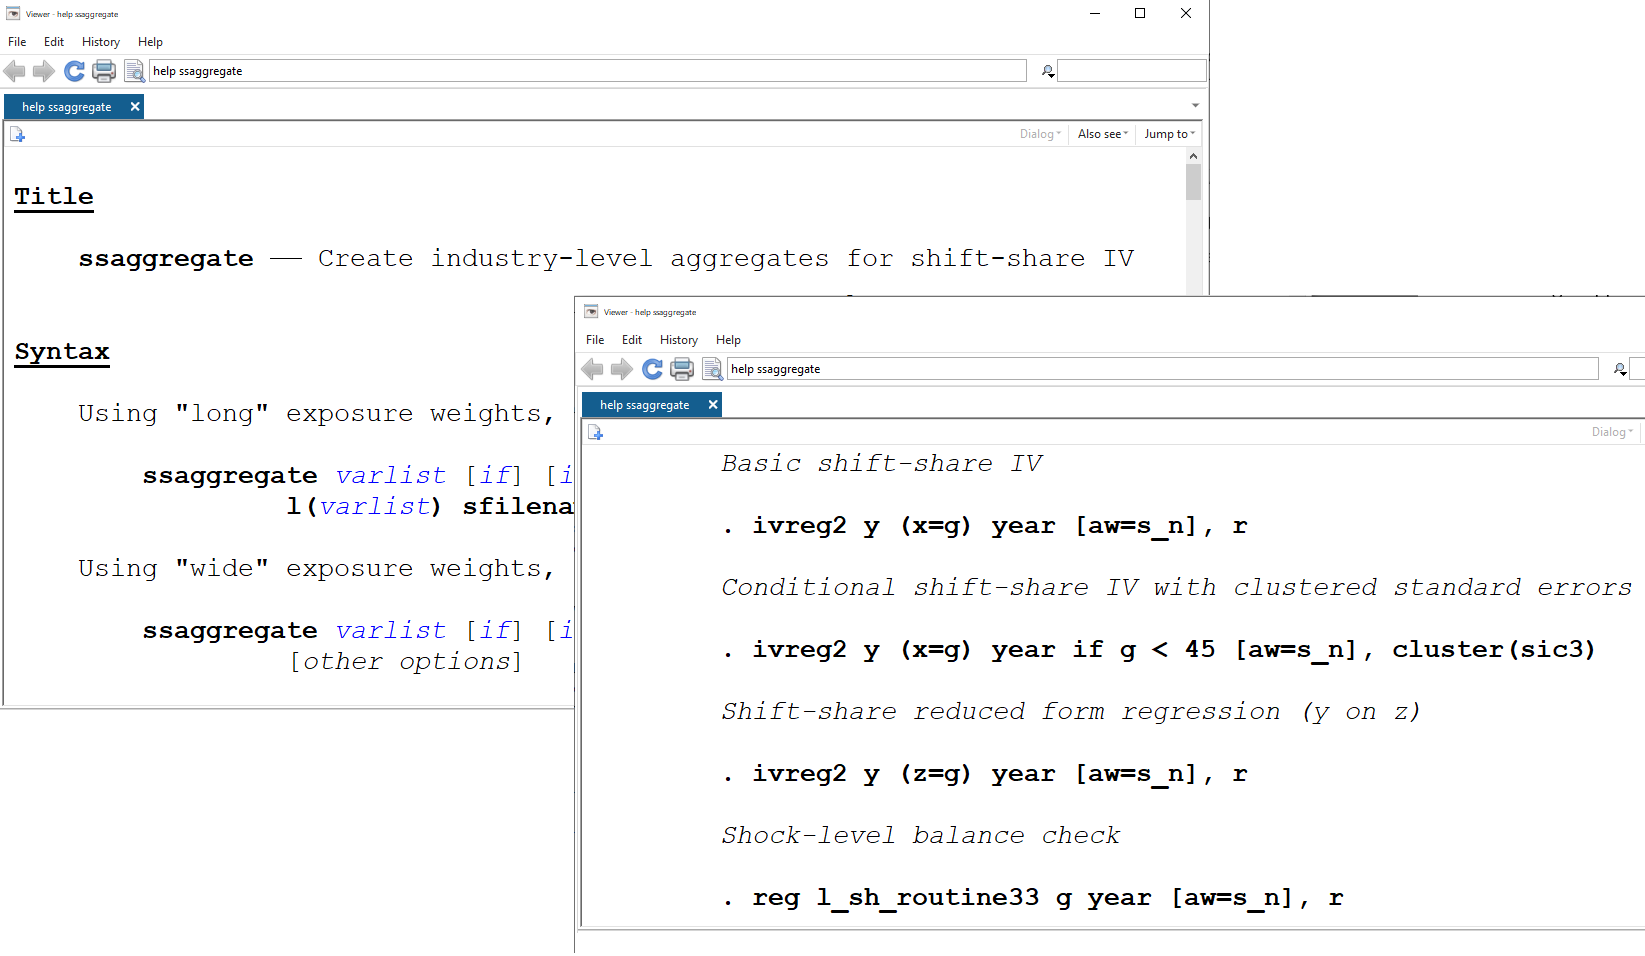
\includegraphics[scale=0.27]{./lecture_includes/ssaggregate.png}
\end{center}
To install: \code{ssc install ssaggregate}
\end{frame}

\begin{frame}{Estimating Exogenous-Shock l SSIV Regressions in R}
\vspace{-0.3cm}
\begin{center}
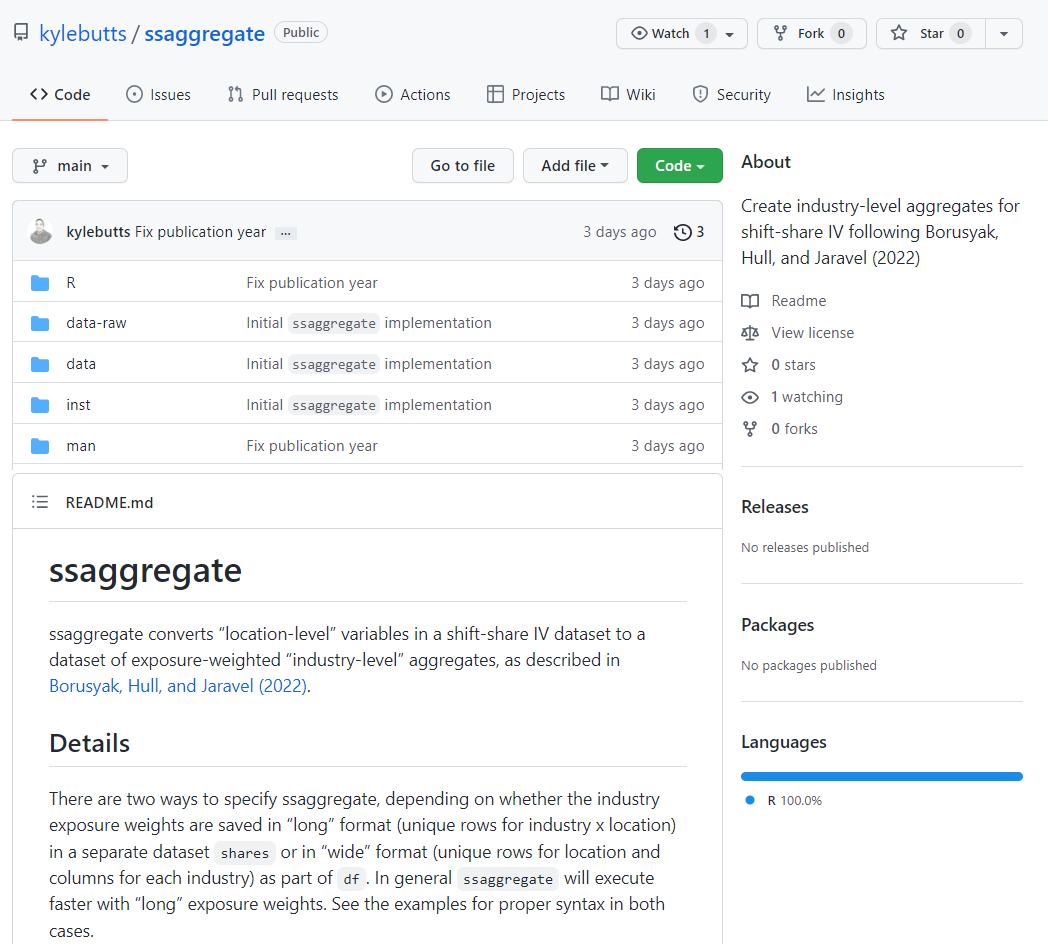
\includegraphics[scale=0.25]{./lecture_includes/ssaggregate_R.png}
\end{center}
\end{frame}

\begin{frame}{For More on SSIV and Related Methods ... }
\begin{center}

\includegraphics[scale=0.4]{./lecture_includes/ssiv_plug.png}
\end{center}
\end{frame}

\section{Other Frontiers}

\subsection{Diff-in-Diff IV}
\begin{frame}{Diff-in-Diff IV}
Remember panel data IVs? We haven't talked about them in a heterogeneous-effects setup but Hudson et al. (2017) do just that\smallskip
\begin{itemize}
\item Intuitively, a LATE interpretation requires parallel trends in both the outcome and the treatment and a subtle exclusion restriction: \\ the IV can only affect outcomes in one period \smallskip
\item This note actually grew out of my Abdulkadiroglu et al. (2016) work
\end{itemize}\bigskip\pause{}

De Chaisemartin and D'Haultfoeuille propose an alternative ``fuzzy difference-in-differences'' approach which makes other assumptions\smallskip
\begin{itemize}
\item Key question is whether you think the RF and FS diff-in-diffs are causal or not (if so, keep calm and \code{ivreg2} on!)
\end{itemize}

\end{frame}

\begin{frame}{The Recent Diff-in-Diff Literature}
You may have noticed there's been, uh, a lot going on with DD recently\smallskip
\begin{itemize}
\item Goodman-Bacon, Sun and Abraham, Callaway and Sant'Anna, Borusyak/Jaravel/Spiess, de Chaisemartin and D'Haultfoeuille ...\smallskip
\item As far as I can tell most/all of this analysis is about ``reduced form'' difference-in-differences
\end{itemize}\medskip\pause{}
My guess is these problems only get worse with IV (work to be done!)\smallskip
\begin{itemize}
\item But presumably if you can use any of these approaches to estimate the RF \& FS, LATE goes through \'{a} la Hudson et al. (2017)\smallskip
\item I don't really have anything smarter to say about that for now...
\end{itemize}
\end{frame}

\subsection{Recentered IV}
\begin{frame}{Recentered IV}
Often we're interested in using instruments that combine multiple sources of variation, only some of which is random \smallskip
\begin{itemize}
\item Network spillover IVs (e.g. Miguel and Kremer 2004)\smallskip
\item Transportation upgrade IVs (e.g. Donaldson and Hornbeck 2016)\smallskip
\item Simulated instruments (e.g. Currie and Gruber 1996)\smallskip
\item Nonlinear shift-share (e.g. Chodorow-Reich and Wieland 2020)
\end{itemize}\bigskip\pause{}

Borusyak and Hull (2021) develop a general identification framework\smallskip
\begin{itemize}
\item Propose ``recentering'' to avoid bias from non-random ``exposure''
\end{itemize}
\end{frame}

\begin{frame}{The Borusyak and Hull (2021) Proposal}
Consider a instrument $Z_i=f_i(g;s)$ for some known mapping $f_i(\cdot)$ of exogenous shocks $g$ and non-random exposure $s$\smallskip
\begin{itemize}
\item BH show that the \emph{expected instrument} $\mu_i=E[f_i(g;s)\mid s]$ is the sole source of bias and the \emph{recentered instrument} $Z_i-\mu_i$ is free of bias
\end{itemize}\medskip\pause{}

$\mu_i$ is measured by taking a stand on the shock \emph{assignment process}\smallskip\pause{}
\begin{enumerate}
\item Specify \emph{counterfactual} shocks $\tilde{g}^{(1)},\dots,\tilde{g}^{(K)}$ which were as likely to have occured (by, e.g., permuting the rows of $g$)\smallskip\pause{}
\item Recompute $Z_i^{(1)},\dots,Z_i^{(K)}$ for each observation $i$: $Z_i^{(k)}=f_i(\tilde{g}^{(k)};s)$\smallskip\pause{}
\item Average the counterfactual instruments for each $i$: $\mu_i=\frac{1}{K}\sum_k Z_i^{(k)}$
\end{enumerate}\medskip\pause{}

Besides recentering, $\mu_i$ can also be controlled for with the original $Z_i$

\end{frame}

\begin{frame}{Illustration: High-Speed Rail in China, 2007-2016}
\vspace{-1cm}
\begin{center}
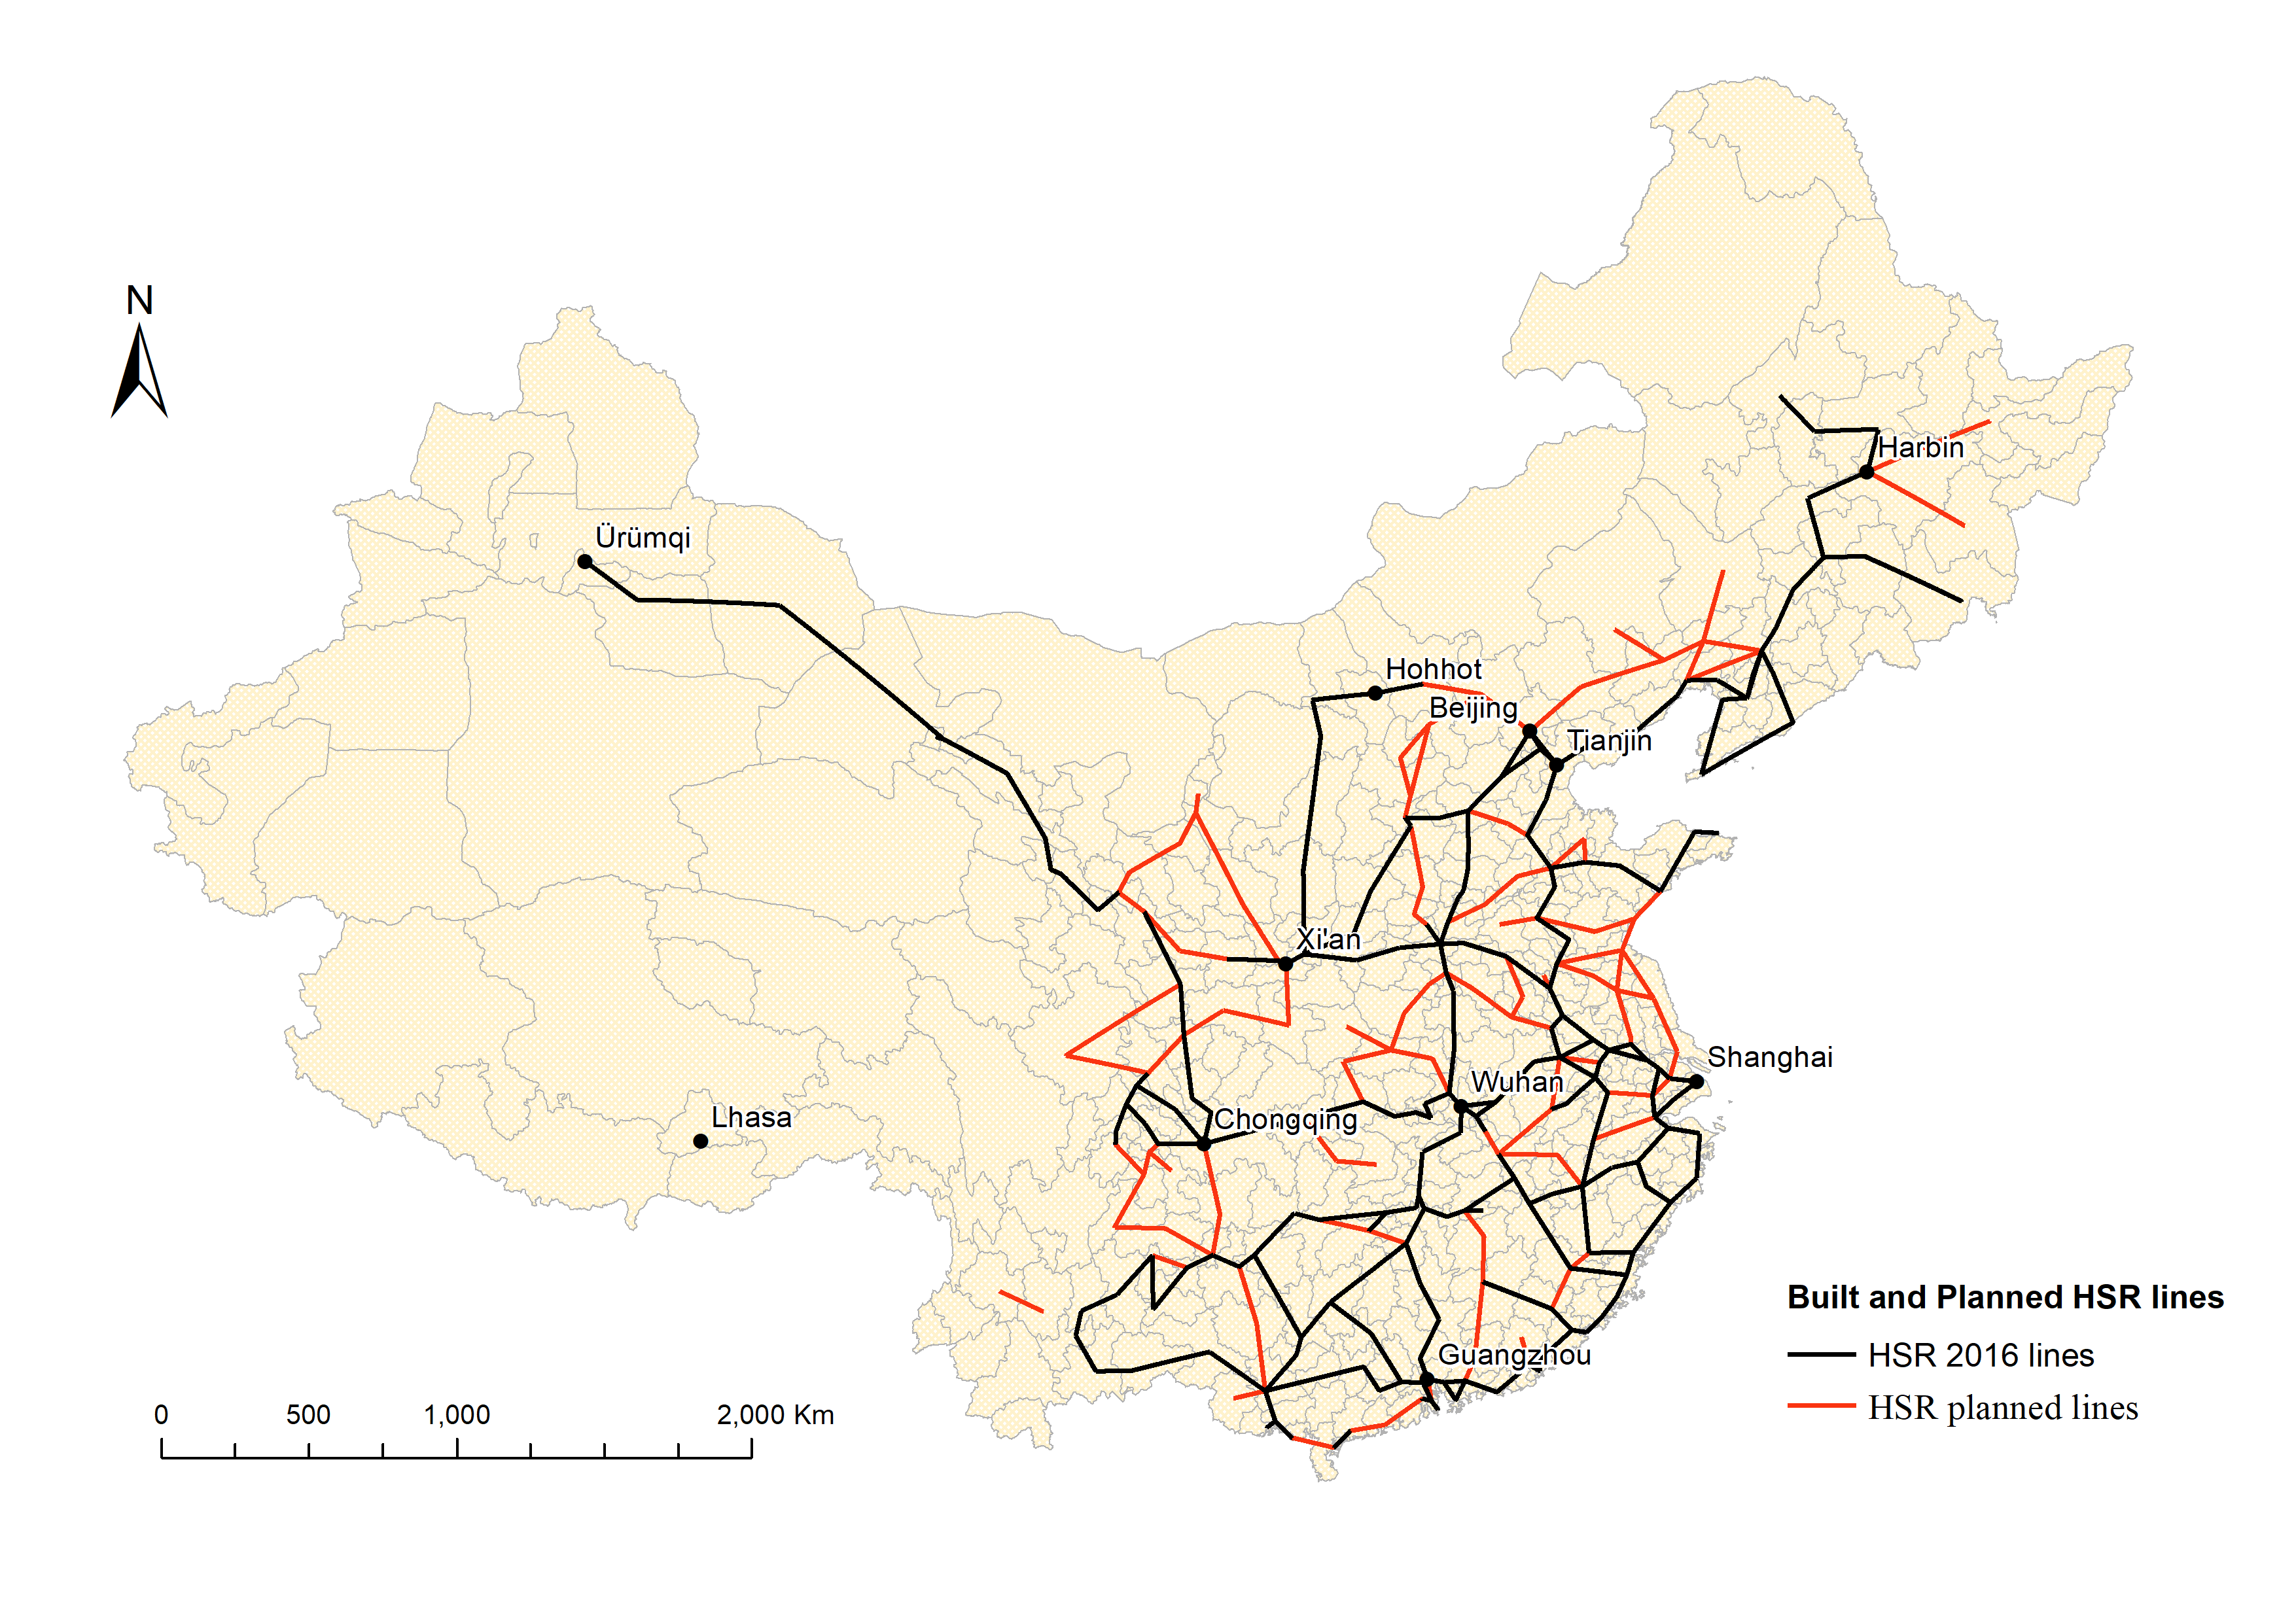
\includegraphics[scale=0.4]{./lecture_includes/Lines_actual_planned.png}
\end{center}

\end{frame}

\begin{frame}{Market Access Growth, Computed from Rail Growth}
\vspace{-1cm}
\begin{center}
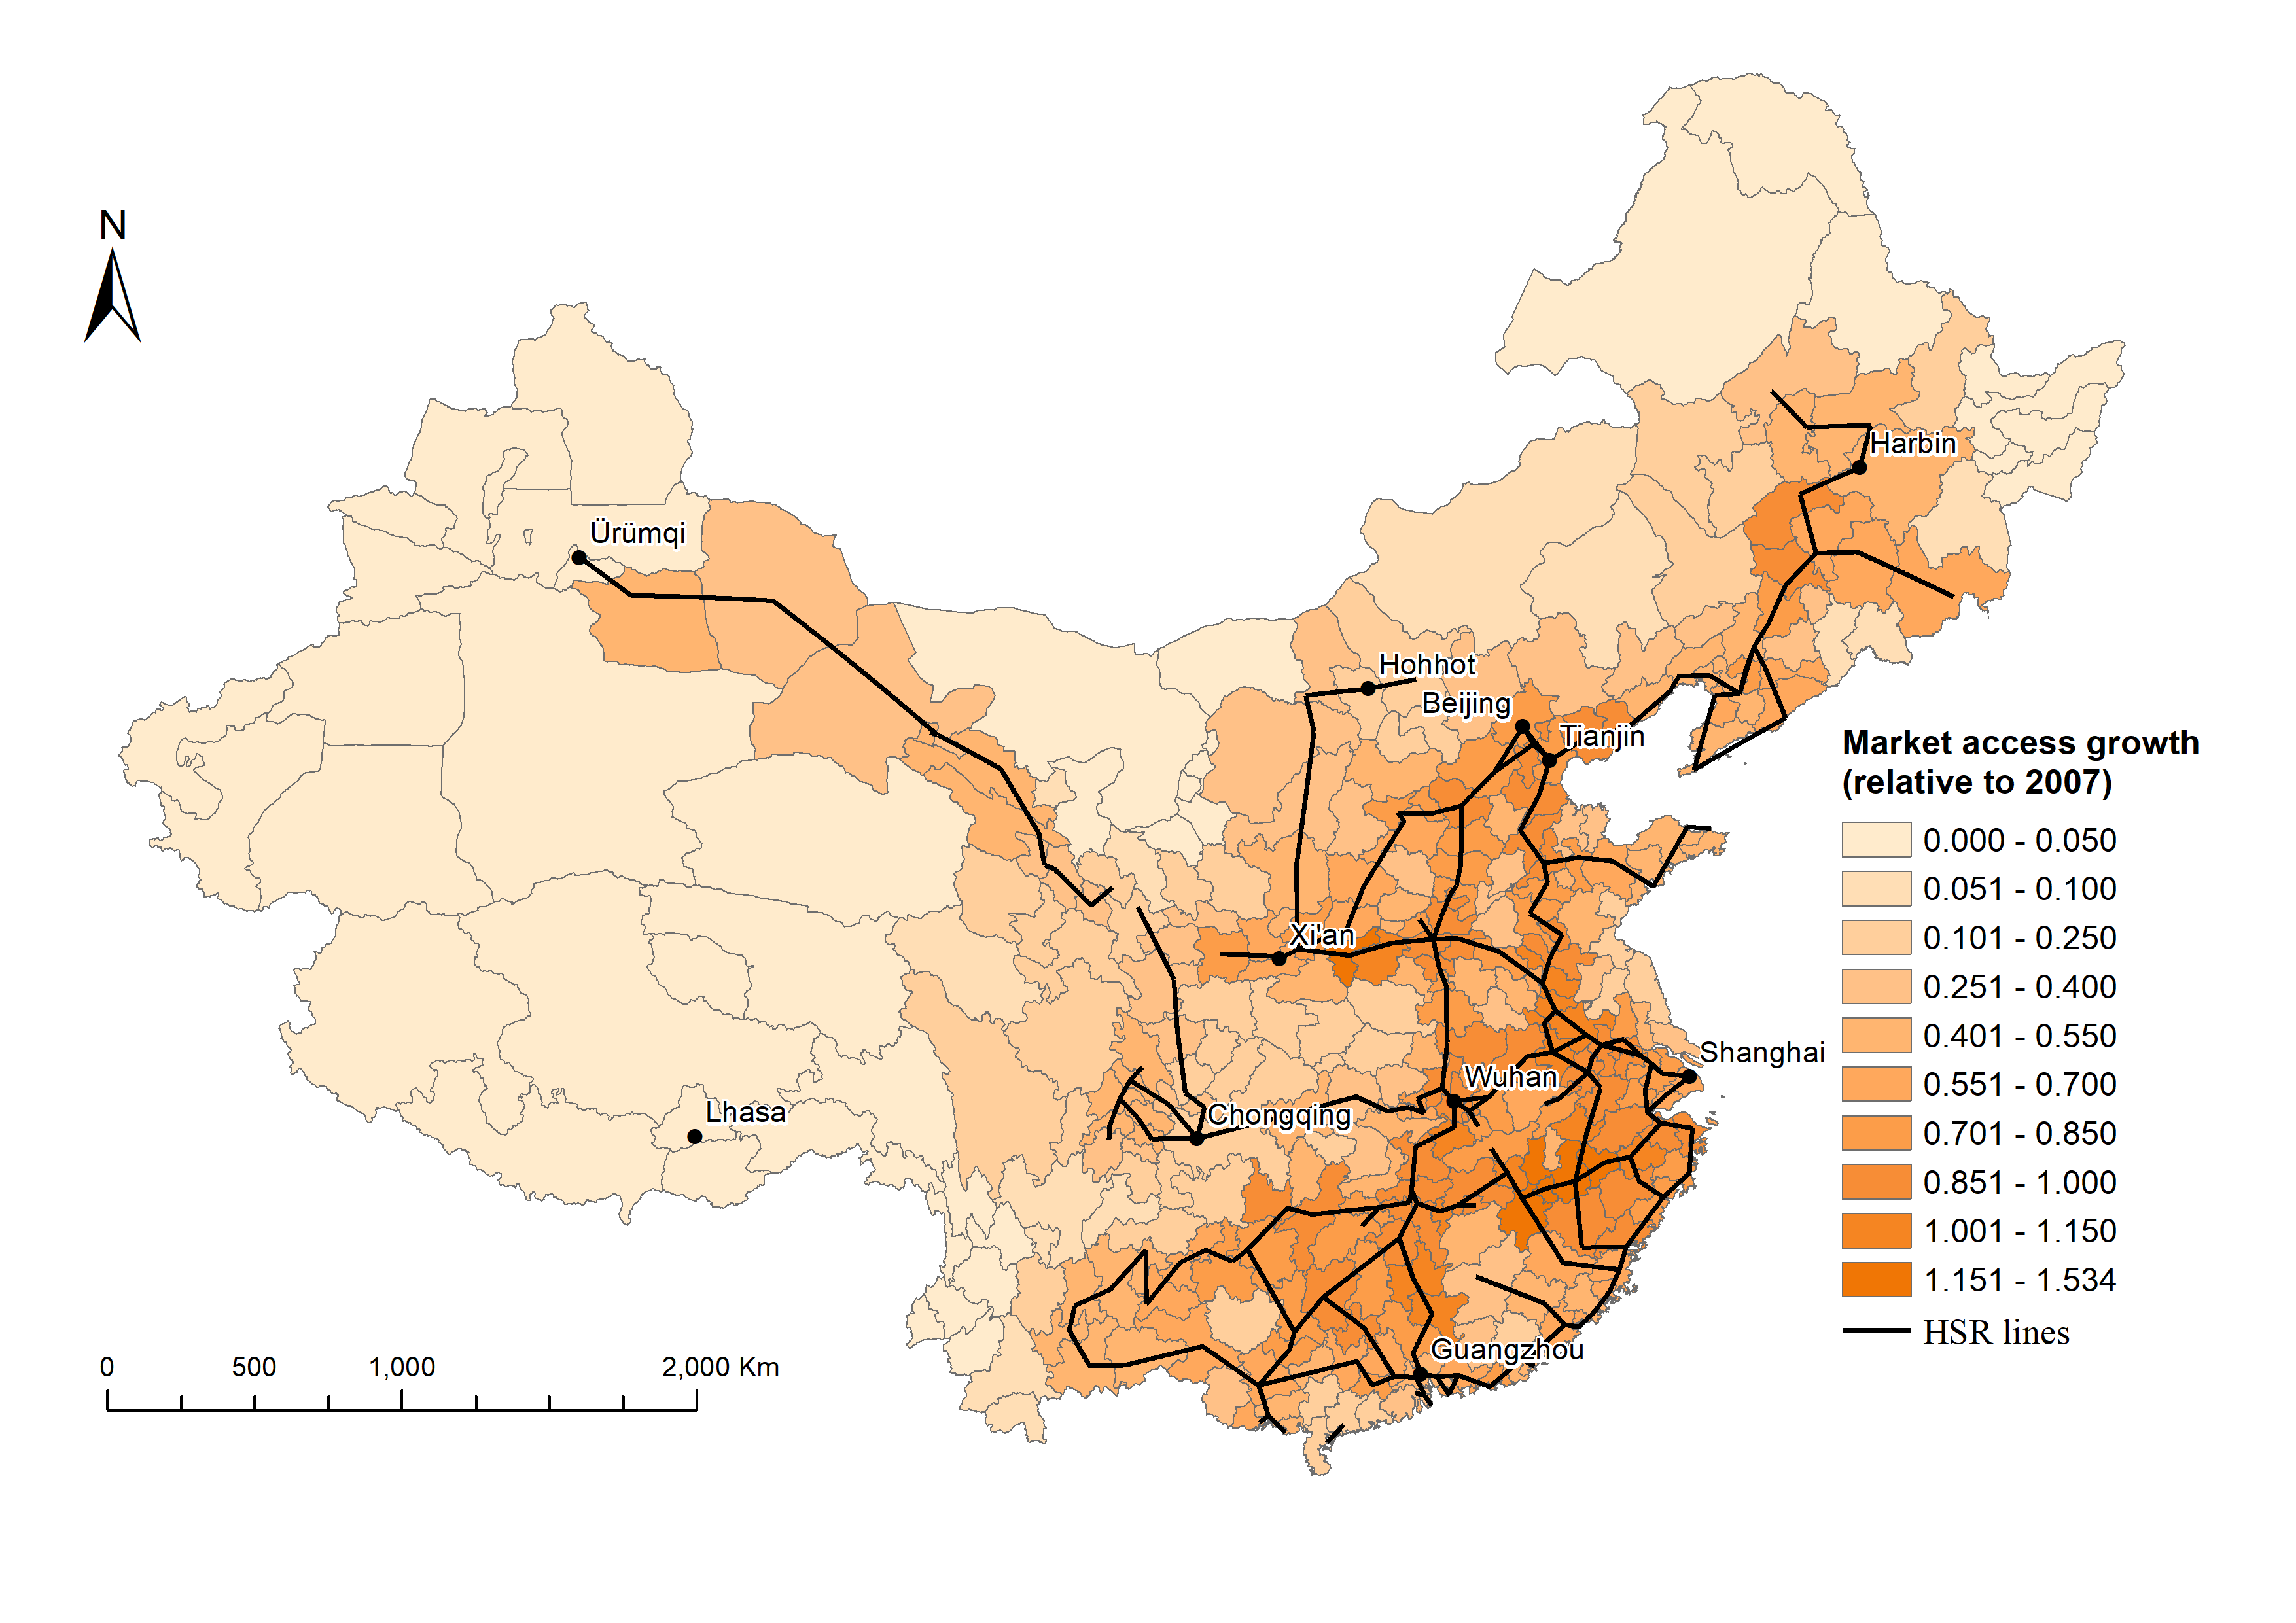
\includegraphics[scale=0.4]{./lecture_includes/Line_panel2016.png}
\end{center}

\end{frame}

\begin{frame}{\emph{Expected} MA Growth, Assuming Random Rail Timing}
\vspace{-1cm}
\begin{center}
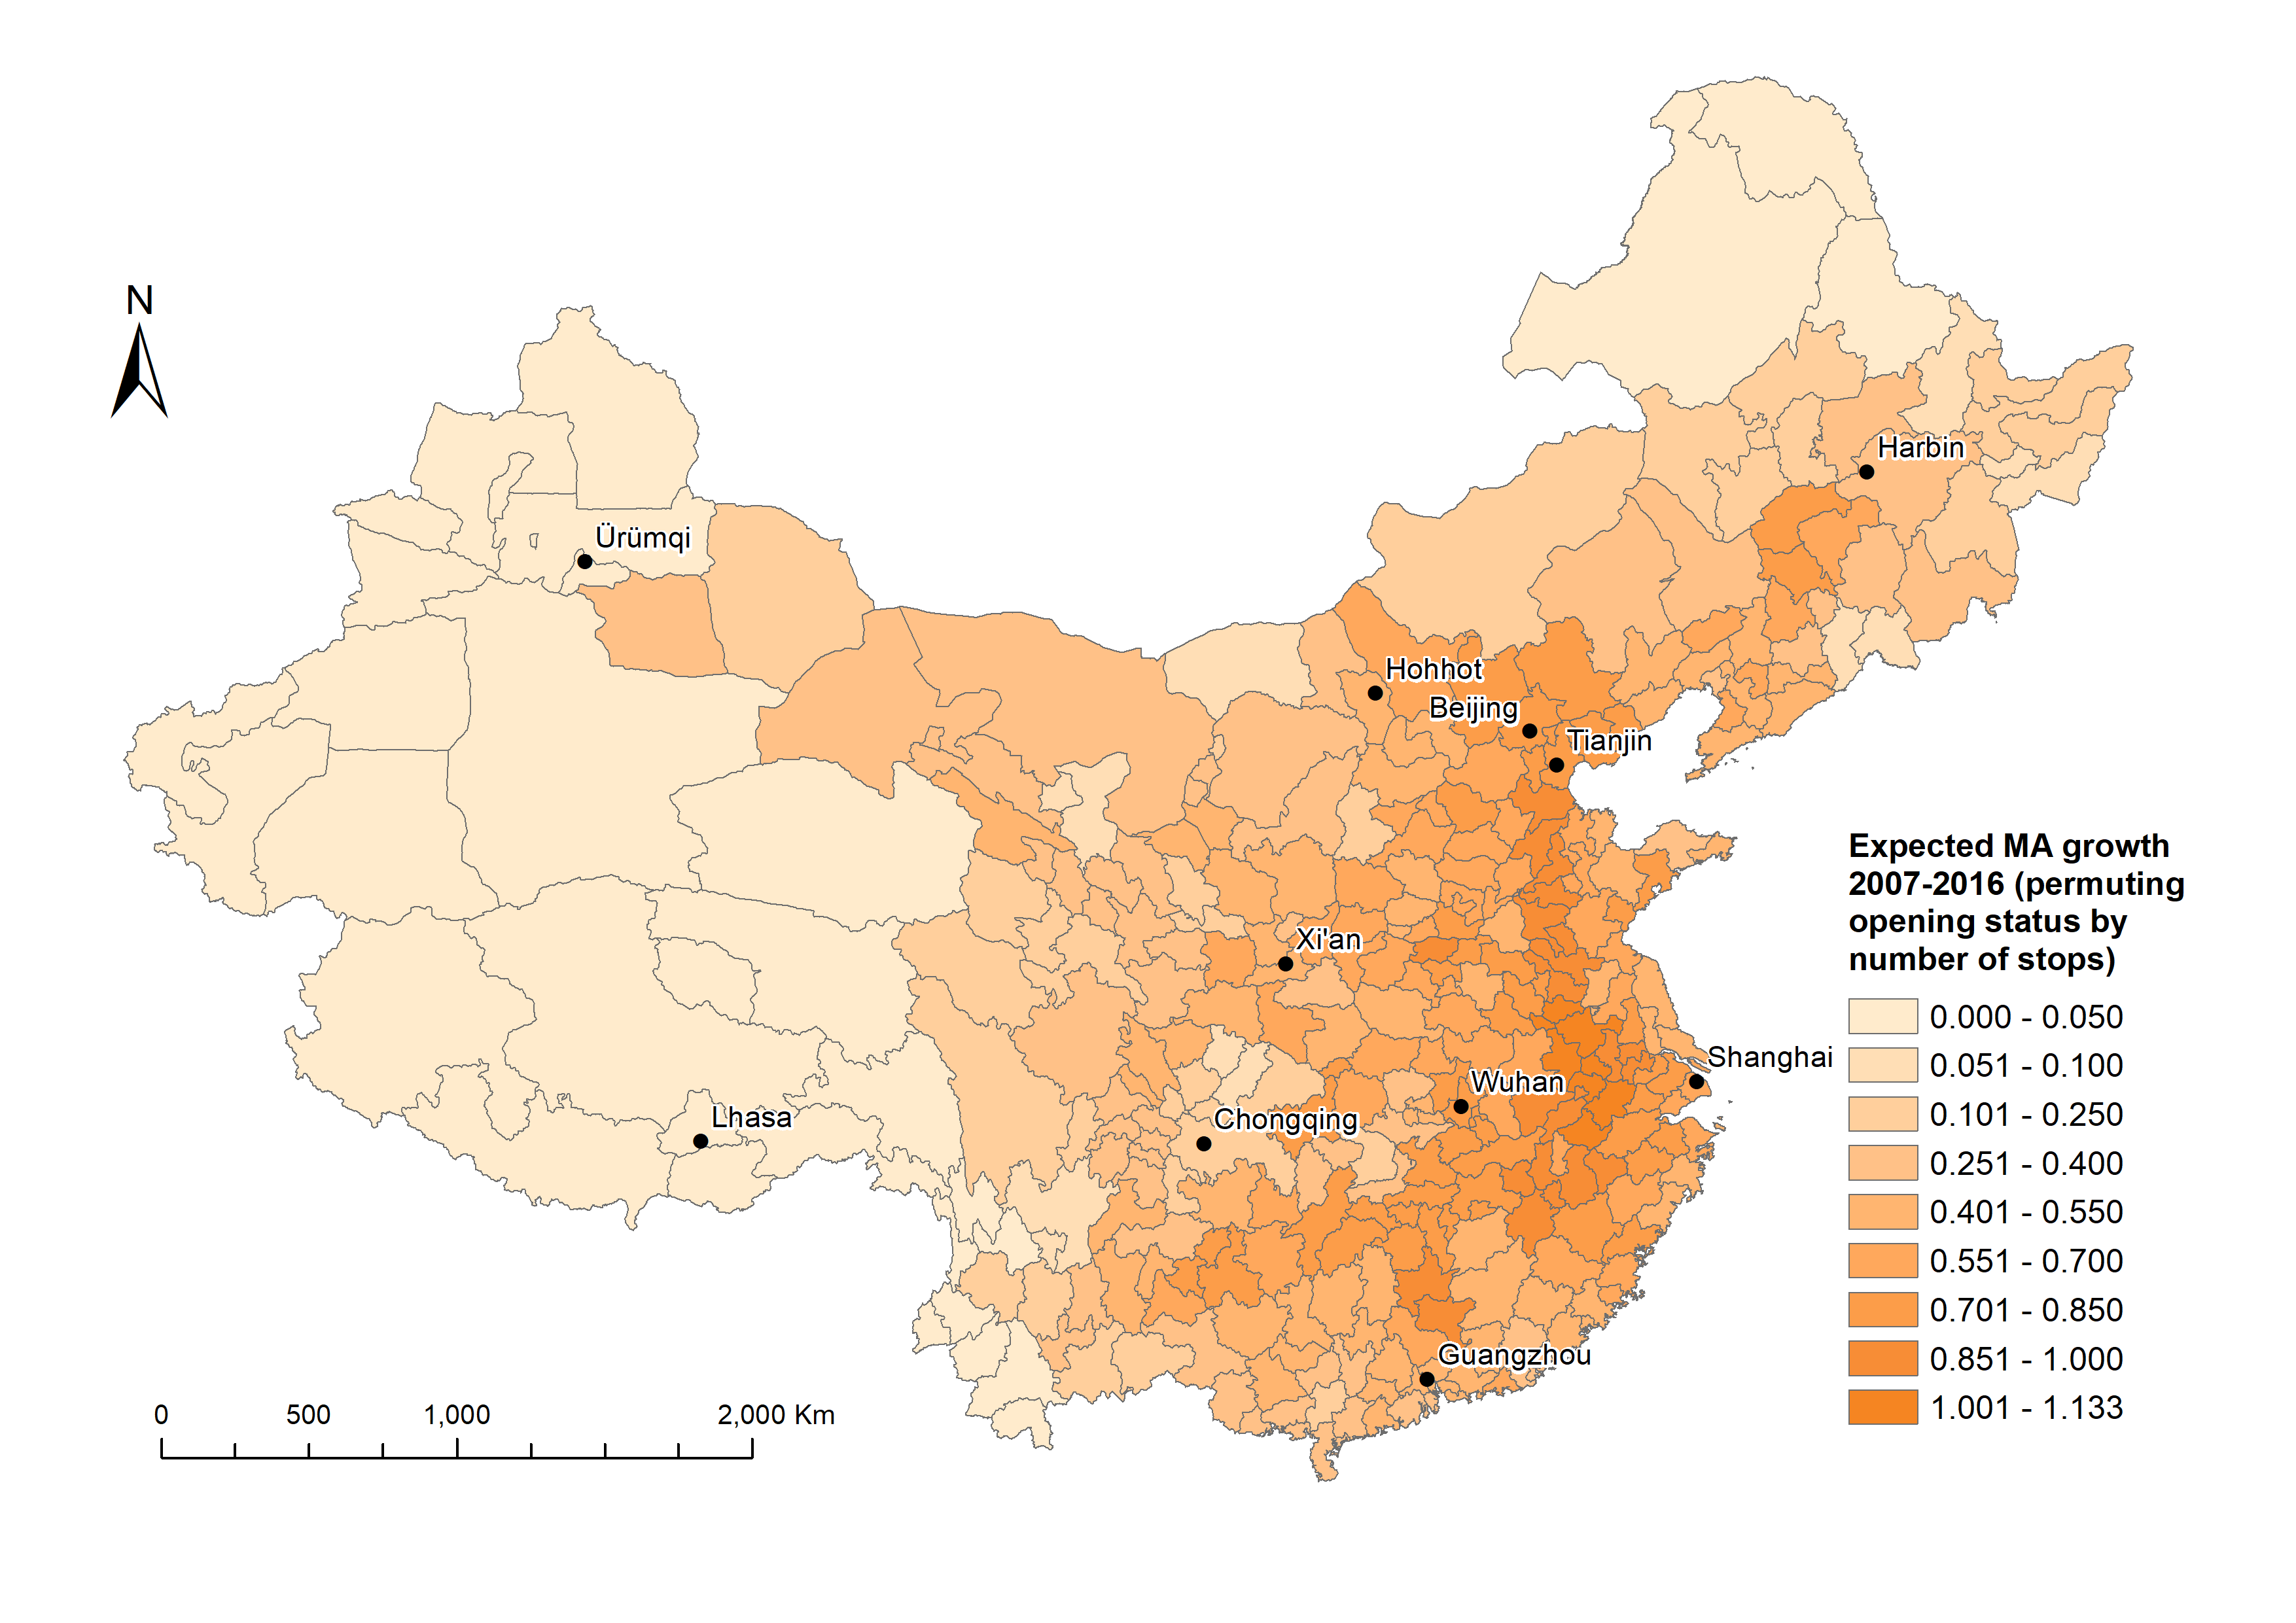
\includegraphics[scale=0.4]{./lecture_includes/NlinkExpected2016.png}
\end{center}

\end{frame}

\begin{frame}{\emph{Recentered} Market Access Growth = Actual - Expected}
\vspace{-1cm}
\begin{center}
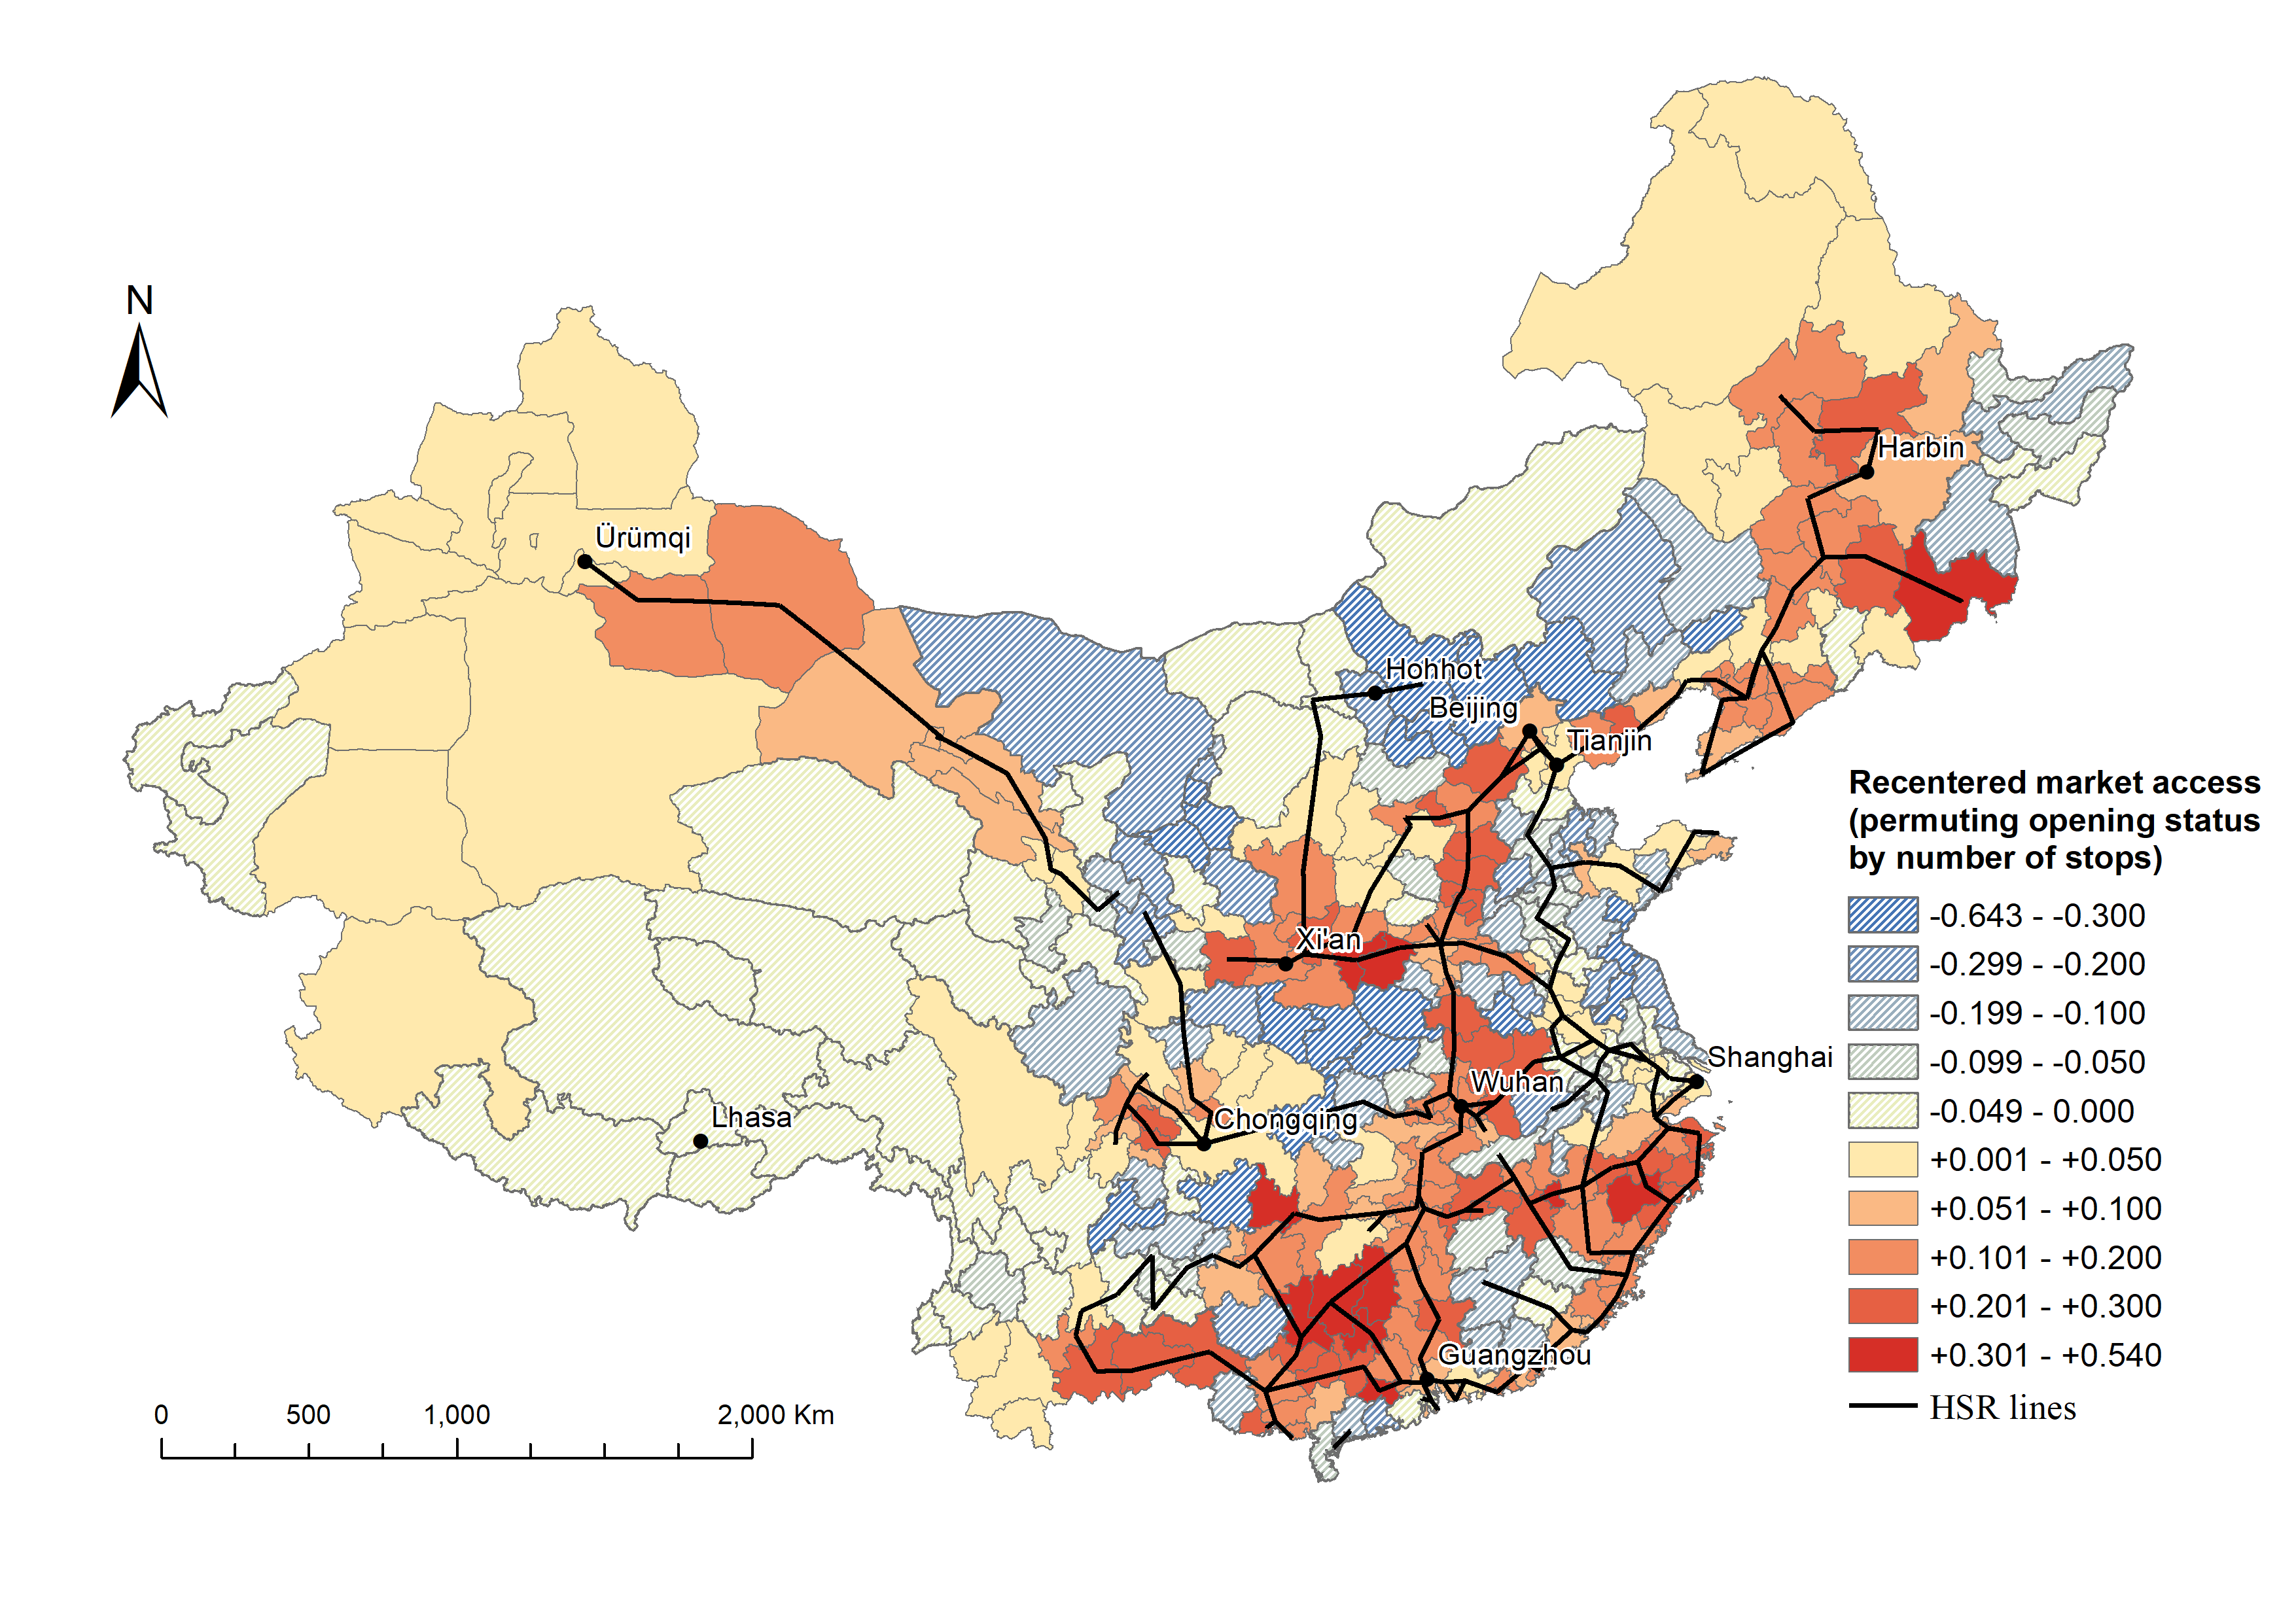
\includegraphics[scale=0.4]{./lecture_includes/NlinkRecentered2016.png}
\end{center}

\end{frame}

\begin{frame}{Recentering Can Matter a Lot Empirically!}

\begin{center}
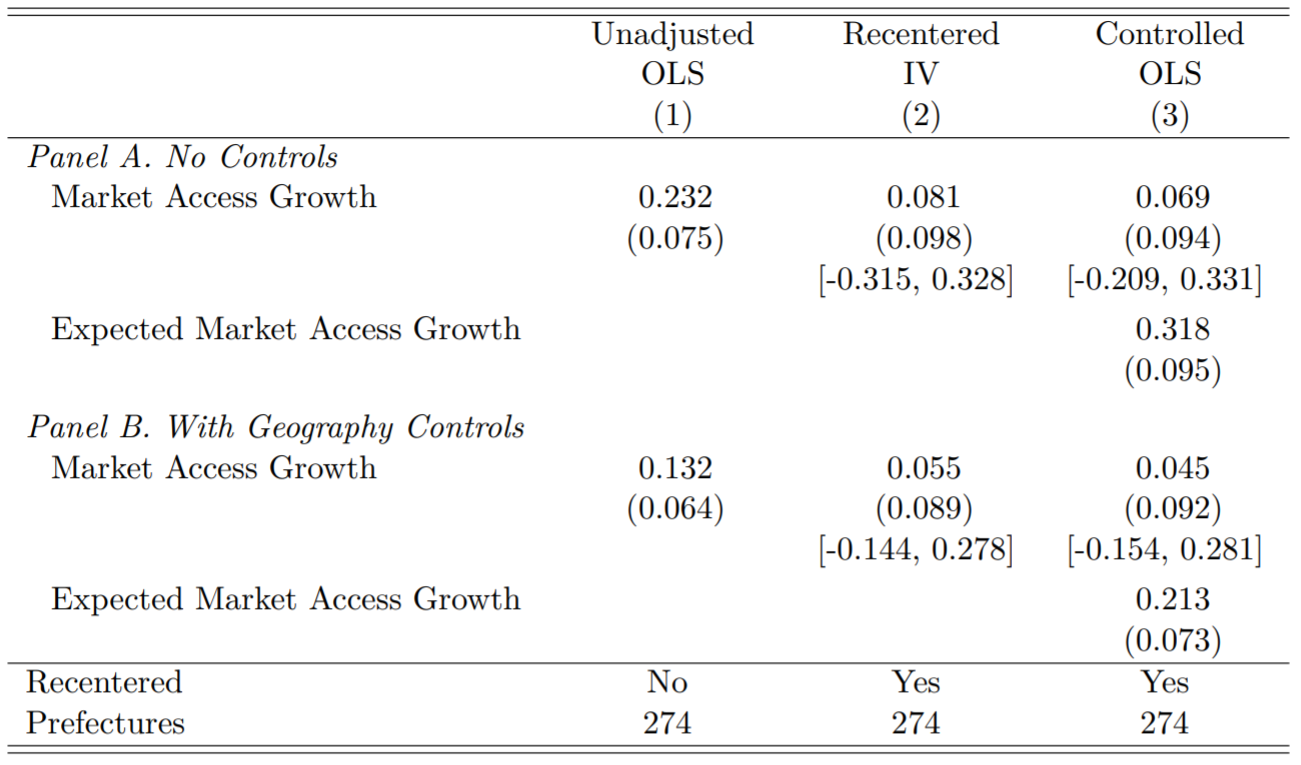
\includegraphics[scale=0.5]{./lecture_includes/hsr_tab.png}
\end{center}
Source: Borusyak and Hull (2021)
\end{frame}

\end{document}
